\section{Experimental Results}
\label{sec:experiments}

\subsection{Bankruptcy prediction}

In this section, we address the problem of predicting the failures of Italian companies. Therefore our interest will be concentrated in predicting which companies will no longer be active in the following year.
Usually in the most important literature on this subject (see for example ~\cite{altman-bankruptcy-17}),  those predictions are performed using primarily balance sheet data. In this work we decided to use the combination of the balance-sheets dataset with the Central Credit Risk. Below in the comments on the results we will focus our attention on the Auroc, which is the performance indicator that we have tried to maximize in setting the algorithms.
The results obtained are shown in the table below: the Auroc, in reaches about 0.9 for the best classifiers and varies slightly depending on the classifier used (0.92 for boosting classifiers while using DT Auroc is 0.77). ML algorithms generally performs better than statistical classifiers like Logistic regression. This result confirms a well known evidence in the recent literature also for our particular dataset.

The overall dataset that we used includes at the beginning approximately 340,000 companies for a total of over 155 columns. Thanks to the use of the Boruta Algorithm for feature selection we succeeded in reducing it to a total of just 12 significant attributes.


\begin{table}[H]
\begin{center}
\begin{tabular}{lcccccccccccl}
\hline
 &AuROC & Recall & Precision  &F1-score & TPR &  TNR\\
\hline
\hline
\LOG         &0.77 &0.58 &0.005       &0.010 &0.38 &0.88 \\
 \hline
\DT         &0.77 &0.75 &0.006       &0.010 &0.78 &0.77 \\
\RF         &0.93 &0.86 &0.008      &0.016 &0.84 &0.83  \\
\CAT        &0.93 &0.88 &0.008       &0.016 &0.85 &0.83 \\
\hline
\\
\end{tabular}
\caption{Balanced training set; balance-sheet data + loan data.}
\label{tbl:bankr_unb_bal}
\end{center}
\end{table}


\subsection{Adjusted default prediction}


In this section we try to predict bank default or more precisely "adjusted default", according to the previous definition (see chapter 3.1).  
\newline
In other words, in this case we will be interested in the prediction of bank default, or in a state of serious difficulty for a company with respect to the banking system, which generally involves the company's inability to repay its bank debts. This condition of a company does not necessarily correspond to a bankruptcy but it is very important to foresee for the stability of the banking and financial system.
\newline
The experimental results are reported in the tables below.
In this case, the usual data used to make prediction are credit data. In our study we used the same merged dataset (credit + balance) as for the bankruptcy problem. 

Also in this case, due to the strong imbalance of the dataset we decided to train all the models on an under sampled dataset. The main performance indicator we have focused our analysis it is the Auroc, but we also looked at other classic indicators including the F1-score.
 We can observe how the Machine learning classifiers have better performance than the other statistical classifiers (for example Logistic Regression). In particular, considering Auroc we can obtain a gain greater than $0.15$. As mentioned before, this result is in line with other evidence in the literature (see in particular Barboza and alt.).


\begin{table}[H]
\small
\begin{center}
\begin{tabular}{lcccccccccl}
\hline
 &AuROC & Recall & Precision  &F1-score & TPR &  TNR\\
\hline
\hline
\LOG          &0.72 &0.66 &0.09       &0.15 &0.67 &0.67 \\\hline
\DT          &0.75 &0.75&0.12       &0.21 &0.74 &0.75 \\
\RF          &0.90 &0.82&0.19      &0.31 &0.83 &0.84  \\
\CAT        &0.91 &0.82&0.20       &0.32 &0.83 &0.84 \\
\hline
\\
\end{tabular}
\caption{Balanced training set;loan+balance data.}
\label{tbl:unb_loan}
\end{center}
\end{table}


Moreover, among the ML classifiers, those that obtain the best results are those of the boosting type with Catboost being the best.
We also found that trying to predict bank default using the combination of the datasets provide improved level of performance .
\newline
Based on this experimental evidence, in this case the conjecture we make is that credit data are critical to predict a bank default while balance sheet data has less predictive power in this case. However, the combination of the two sources of information can improve adjusted default prediction.


\subsection{Adjusted default prediction with AnaCredit data}

In this section, we show the first evidence using a new credit dataset from AnaCredit survey. The main results underline that the new data have good forecasting capabilities, similar to the CR loans data used in the previous predictions. We can obtain using AnaCredit data in combination with Central Credit Register data Auroc equals to $0,93$ for the best classifier.



\begin{table}[H]
\begin{center}
\begin{tabular}{lcccccccccccl}
\hline
 &AuROC & Recall & Precision  &F1-score & TPR &  TNR\\
\hline
\hline
\LOG         &0.86 &0.87 &0.05       &0.10 &0.80 &0.66 \\
 \hline
\DT         &0.78 &0.78 &0.07       &0.12 &0.79 &0.78 \\
\RF         &0.92 &0.83 &0.11      &0.19 &0.84 &0.86  \\
\CAT        &0.93 &0.84 &0.11       &0.19 &0.84 &0.86 \\

\hline
\\
\end{tabular}
\caption{Balanced training set; Anacredit + Central Credit Register.}
\label{tbl:unb_anac}
\end{center}
\end{table}




The complete dataset consists of $573,000$ rows and $136$ columns that after feature selection is reduced to $16$ .
Since the AnaCredit dataset is very recent (starting from September 2018) in this exercise we will use data relating to the last few years (from 2019 to 2020). It will therefore not be possible to use balance sheet data as these are not yet available.



\subsection{Evaluation of results: default prediction based on banks Probability of Default}

In order to evaluate the performance of Machine learning classifiers, we would compare the previous predictions with a prediction performed using the "Probability of default" that is reported from the Italian banks in AnaCredit. In particular we assume that we will predict a default if a firm has a probability of default greater than an established threshold.
The prediction results show a very low performance demonstrating the difficulty of the default prediction problem. The best prediction results we obtain are in correspondence with the PD threshold equal to 0.1 (i.e. assuming as default the companies that the previous year have a PD greater than 0.1) but also in this case it is not possible to obtain an Auroc greater than 0.7.


\begin{figure}[H]

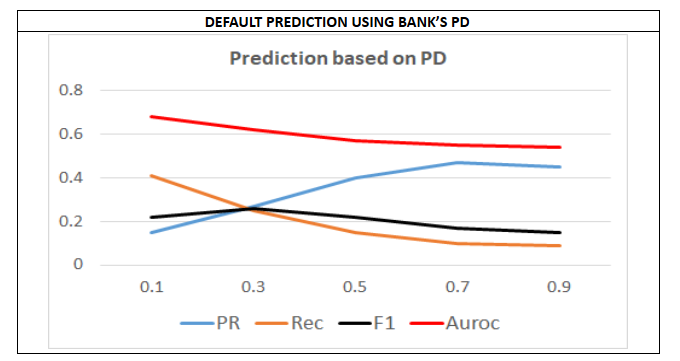
\includegraphics[width=120mm, height=80mm]{figs/PD.png}

\caption{Adjusted default prediction based on bank's PD}
\end{figure}

As we have seen above, the Probability of Default is one of the most relevant forecasting factors even using ML algorithms. But the use of these techniques, in particular the tree-ensemble algorithms, provide a significant performance gain with an Auroc higher than 0.93.


\subsection{Explainability}
In this section we use SHAP in order to show an analysis of the predictions regarding both Bankruptcy and Adjusted default.

\paragraph{Bankruptcy}

We analyze Bankruptcy predictions that we obtained using the combination of balance sheet data and credit data. In this case we consider our best performing model CatBoost.
From the explanatory overview we can observe the most important features that determine the forecast: the "rating" appears to be the most relevant one together with other features (X20-"EBITDA/Net financial charges" and X14-"MOL/operational added value") from the balance sheet dataset, but also the overdrafts ("scoperto") also plays an important role.

Usually bankruptcy predictions are made using only balance sheet attributes, from our overview we can definitely say that credit data can really be meaningful with a clear explanatory power even though balance are still the most of the important attributes.

\begin{figure}[H]
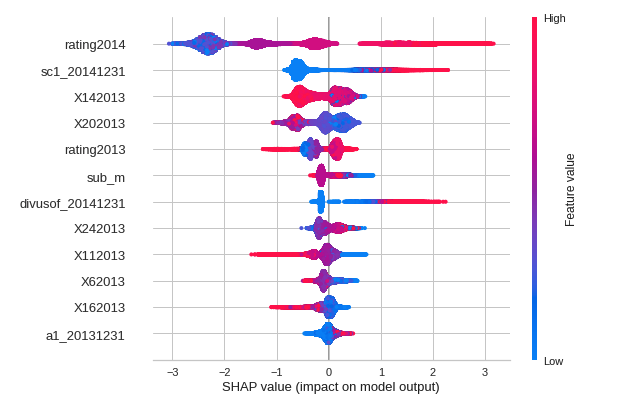
\includegraphics[scale = 0.7]{latex/figs/bankrupt_exp.png}
\caption{Explanatory overview Catboost}
\end{figure}

SHAP values allows us to see also in detail the effect of each attribute on a single prediction.
In the example below we can see how the prediction of an healthy organization is primarily driven by a very low rating bot in 2014 and 2013 and an overdraft equal to zero.
\begin{figure}[H]
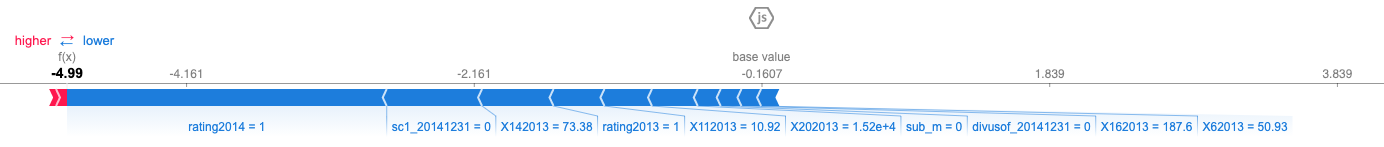
\includegraphics[scale=0.4]{latex/figs/bankrupt1_exp.png}
\caption{Explanation of a single negative prediction}
\end{figure}
In this other example instead is possible to see that the prediction of this firm as failed is due to the high rating in 2014 and 2013 while at the same time to the high overdraft and the decrease over the year of its margins.
\begin{figure}[H]

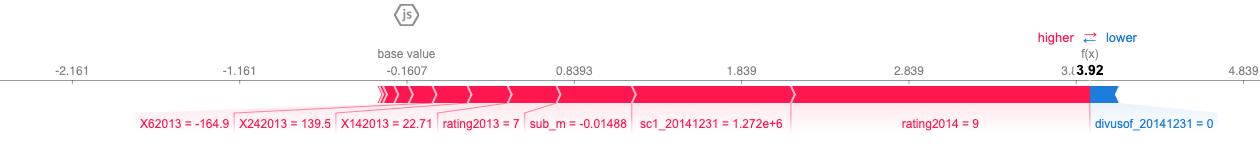
\includegraphics[scale=0.4]{latex/figs/bankrupt2_exp.png}
\caption{Explanation of a single positive prediction}
\end{figure}


\paragraph{Adjusted default}

Considering Adjusted default prediction, we first consider the prediction exercise we conducted using both the balance sheet and credit datasets. An analysis of the results obtained using the CatBoost classifier are shown in the following figures. Also in this case if we use other classifiers we obtain similar results. 
We can see that the most important features in prediction are again "rating" (that shows an important predictive power also for bank default) but some credit features appear decisive such as the overdraft "scoperto" (sc) and "previous default status" (pos).  
This analysis corroborates our conjecture that to predict credit default, credit data are fundamental but at the same time some balance sheet features can also improve bank default forecasts and provides a clear intepretability.


\begin{figure}[H]

%\flushleft
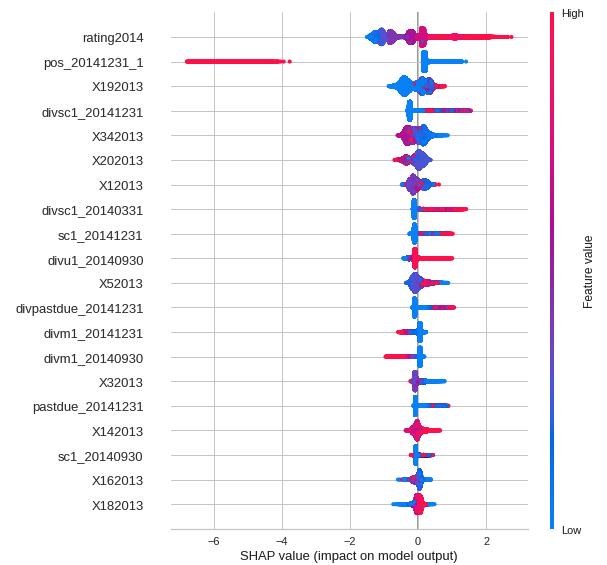
\includegraphics[scale = 0.7]{latex/figs/adjusted_exp.png}
\caption{Explanatory overview Catboost}
\end{figure}

As for the bankruptcy prediction we show how the SHAP values for both healthy and failed companies provide a clear picture of the reasons why that prediction has been made, accordingly to the explanatory overview.
\begin{figure}[H]
\flushleft
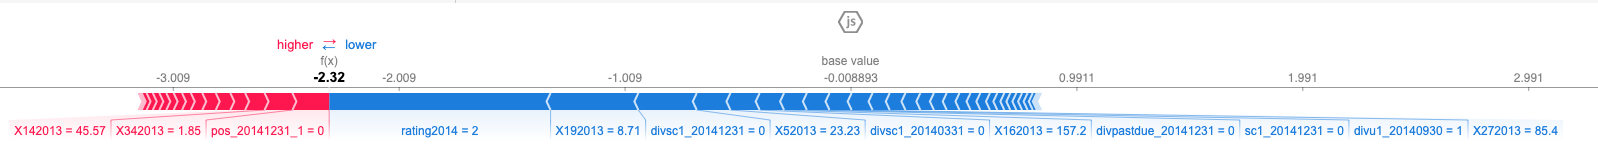
\includegraphics[scale=0.4]{latex/figs/adjusted1_exp.png}
\caption{Explanation of a single negative prediction}
\end{figure}

\begin{figure}[H]

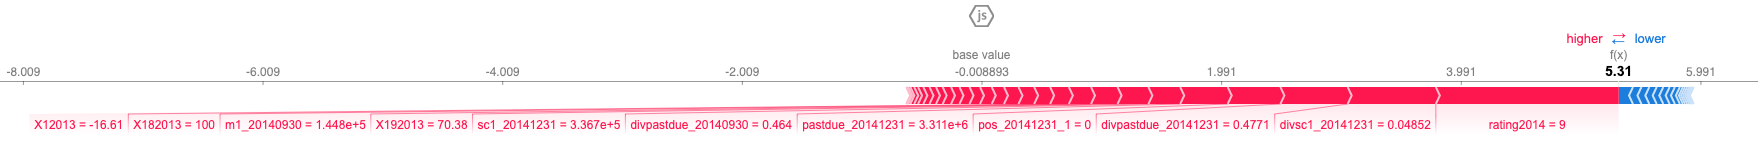
\includegraphics[scale=0.28]{latex/figs/adjusted2_exp.png}
\caption{Explanation of a single positive prediction}


\end{figure}

Finally we consider Adjusted default prediction using only credit data for  the most recent period in which no balance sheet data are available. An analysis of the results obtained using the Catboost classifier are shown in the following figures. Also in this case if we use other classifiers we obtain similar results. We can see that in this case there is a nice balance between the feature of the two datasets. The dominant elements are the probability of default, Unlikely To Pay (inadprob), arrears and the ratio of overdraft over the granted amount (divsc)


\begin{figure}[H]
%\flushleft
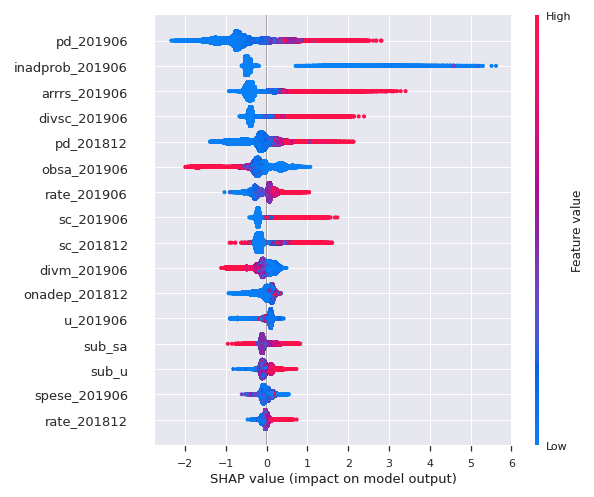
\includegraphics[scale = 0.6]{latex/figs/anac_exp.png}

\caption{Explanatory overview Catboost}
\end{figure}
\begin{figure}[H]
%\flushleft
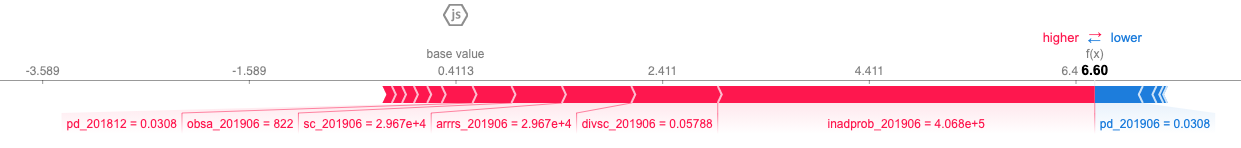
\includegraphics[scale = 0.3]{latex/figs/anac_exp2.png}

In this single prediction explanation is important to notice how despite the fact that the company has the most important attributes, the probability of default, very low it succeed in predicting the company properly basing it on all the other features and showing how they influenced it. 
\caption{Explanation of a single positive prediction}
\end{figure}
\begin{figure}[H]
%\flushleft
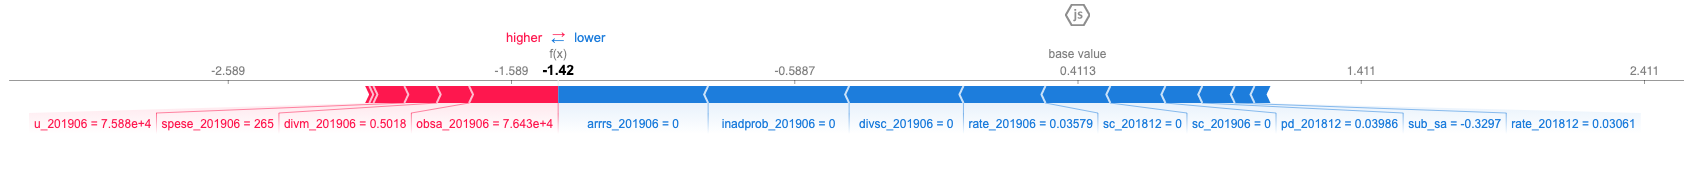
\includegraphics[scale = 0.3]{latex/figs/anac_exp1.png}

\caption{Explanation of a single negative prediction}
\end{figure}

The analysis carried out with SHAP clearly shows some features that are dominant in the forecasts and that belong to both the balance sheet and credit dataset. It seems relevant to us to underline that all these factors can be correlated with potential problems of the company that may be detectable in periods prior to the firms failure.







